\documentclass[12pt]{article}
\usepackage{../../../assignment}
\usepackage{../../../math}
\usepackage{../../../uark_colors}
\hypersetup{
  colorlinks = true,
  allcolors = ozark_mountains,
  breaklinks = true,
  bookmarksopen = true
}

\begin{document}
\begin{center}
  {\Huge\bf Midterm - Fall 2025}

  \smallskip
  {\large\it ECON 5783 — University of Arkansas}
\end{center}

\medskip
\begin{enumerate}
  \item Say a researcher wants to model the conditional expectation
    of European soccer team performance given total annual player
    salary and country.
    \begin{enumerate}[label=(\alph*)]
      \item They regress 10-year win percentage on a set of indicator
        variables for each European country and a linear term for
        total salaries paid.
        Give two limitations of this model % and recommend a way to
        % fix each limitation.
    \end{enumerate}

    \bigskip\bigskip
  \item A researcher wants to estimate the effect of taking vitamin
    supplements on health outcomes.

    \begin{enumerate}[label=(\alph*)]
      \item Do you think the difference-in-means estimate will
        identify the causal effect of supplements?
        If not, predict the sign selection bias and explain your thinking.

      \item The researchers are aware of this problem and therefore
        use a selection on observables identification strategy.
        They condition on age and self-reported diet quality.
        Describe in your own words what the conditional independence
        assumption is assuming here

      \item Give an example of why the causal assumption might fail.

      \item Assume that you think the \emph{causal} assumption holds.
        For each of the following estimation strategies, write what a
        researcher needs to worry about: (i) regression adjustment,
        (ii) inverse probability of treatment weighting, (iii)
        aggregating sub-sample ($\bm{X}_i = \bm{x}$) difference-in-means
    \end{enumerate}
\end{enumerate}

\newpage
\noindent
% https://arxiv.org/pdf/2508.02658v1
The following questions refer to new work by Feng and Ruggieri (2025).
These authors use a regression discontinuity design to estimate the
housing price effect of school district finance referendums passing.
They look at narrowly winning and narrowly losing elections on home
prices 5 years later (to allow time for capitalization).
See the following figure for their main estimate

\begin{figure}[!b]
  \centering
  \caption{RDD Estimates}
  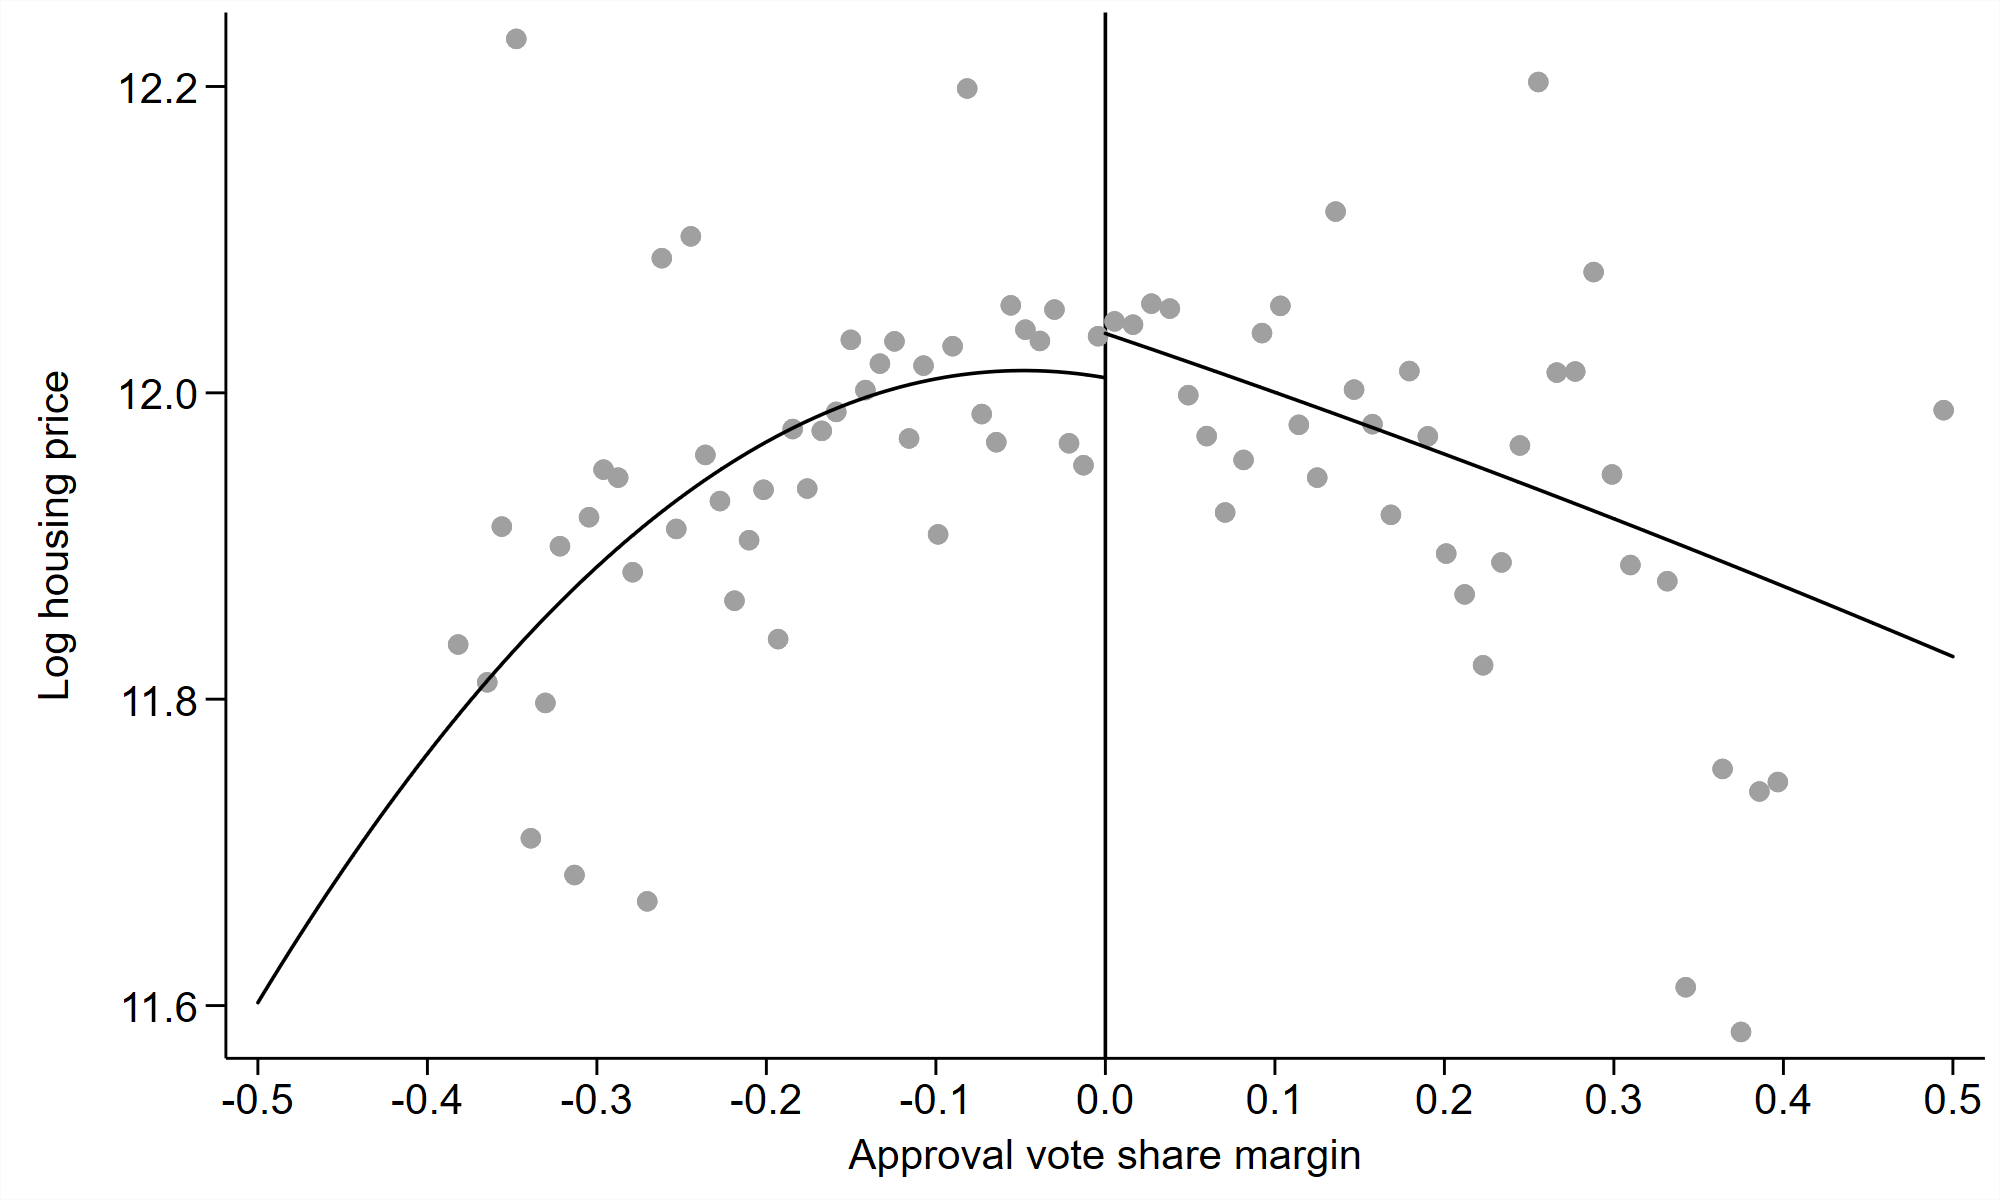
\includegraphics[width=0.85\textwidth]{Feng_Ruggieri_2025.png}
\end{figure}

\begin{enumerate}
    \setcounter{enumi}{3}
  \item What do the authors need to assume for the RDD estimate to be
    interpreted as causal?
    Argue why this might be plausbile in the context of referendum vote share.

  \item The authors do not include data for referendum that are
    raised multiple years in a row by the same district.
    Why might including those elections create problems with the
    causal assumption you discussed in the previous question?

  \item In class we discussed that RDD identifies the LATE (Local
    ATE) for disctricts at the 50\% vote cutoff.
    Given this, why might we think the effects for this group differ
    from districts where the referendum passes by large margins.
\end{enumerate}

\newpage
\noindent
The following questions refer to the paper Systemic Discrimination
Among Large U.S. Employers by Kline, Rose, and Walters (2022, QJE).
The authors ran a large-scaled randomized experiment `sending more
than 83,000 fictitious applications with randomized characteristics
to geographically dispersed jobs posted by 108 of the largest U.S. employers.'
For each application, they randomly changed the applicant to have
`distinctivly Black' or `disctinctivly White' names.
They find that on avereage `Distinctively Black names reduce the
probability of employer contact by 2.1 percent-age points relative to
distinctively white names.'

\bigskip
\begin{enumerate}
    \setcounter{enumi}{6}
  \item Say the authors instead only had a non-experimental sample of
    workers' applications and whether or not they received an employer callback.
    Why might the difference in callback rate between Black and White
    workers not be completely explained as the ``causal discriminatory effect''?

  \item The authors include table 1 in the paper summarizing
    information from the applications they send.
    Why do you think they include this table?

  \item The paper then tries to estimate firm-specific discrimination
    estimates (firm-specific difference in callback rate).
    This results in many different "small experiments" for each individual firm.
    Say a newspaper wanted to take the estimates from this and label
    `the 5 most discriminatory firms'.
    Why might you caution this reporter of selecting the most
    discriminatory estimates?
\end{enumerate}

\begin{table}[!b]
  \centering
  \caption{Characteristics of Applications}
  \begin{tabular}{lccc}
    \toprule
    & {\small`Distinctively White' } & {\small`Distinctively Black' Names} & \\
    & {\small Names} & {\small Names} & {\small Difference} \\
    \midrule
    Résumé characteristics \\
    \quad Female & $0.500$ & $0.498$ & $0.003$ \\
    \quad Over 40 & $0.534$ & $0.533$ & $0.002$ \\
    \quad LGBTQ club member & $0.079$ & $0.080$ & $-0.001$ \\
    \quad Academic club & $0.039$ & $0.042$ & $-0.003^{*}$ \\
    \quad Political club & $0.042$ & $0.041$ & $0.001$ \\
    \quad Gender-neutral pronouns & $0.040$ & $0.040$ & $0.000$ \\
    \quad Same-gender pronouns & $0.042$ & $0.041$ & $0.001$ \\
    \quad Associate degree & $0.478$ & $0.485$ & $-0.006^{*}$ \\
    \bottomrule
  \end{tabular}
\end{table}

\end{document}
